\section{Project 4 - Image Restoration}
\subsection{Project Proposal}
First implement the random noise generation functions. The random noise functions include uniform, Gaussian, Rayleigh, Gamma, exponential and impulse. Requirement is that only uniform noise is allowed to use built-in function while any other noise should be generated based on uniform noise with self-defined functions. The test image is \emph{Fig0503.tif}.
Second follow the process shown in textbook \emph{FIGURE 5.7, FIGURE 5.8, FIGURE5.9, FIGURE 5.10, FIGURE 5.11, FIGURE 5.12}. Each figure displays a process of add some specified type of noise and then use restoration method to reduce noise.

\subsection{Preliminaries}
\subsubsection{Noise Models}
The principal source of noise in digital images arise during image acquisition and/or transmission. We assume in this project that noise is independent of spatial coordinates and uncorrelated with respect to the image itself. Thus, what we concerned is the statistical behavior of the intensity value in the noise component which can be described by PDF.\\ 
\textbf{Uniform distribution}
\begin{equation} p(z)=\left\{ \begin{array}{crl} \frac{1}{b-a} & a\leq z \leq b \\ 0 & \text{otherwise} \end{array} \right. \end{equation} \begin{equation} E(z)=\frac{b-a}{2}, ~~~~ Var(z)=\frac{(b-a)^2}{12} \end{equation}
In the process of generating other distribution, we usually use $a=0$ and $b=1$. \\
\textbf{Gaussian distribution}
\begin{equation}p(z)=\frac{1}{\sqrt{2\pi}\sigma}e^{-(z-\mu)^2/2\sigma^2} \end{equation} \begin{equation} E(z)=\mu, ~~~~ Var(z)=\sigma \end{equation}
\textbf{Rayleigh distribution}
\begin{equation} p(z)=\frac{z-a}{\sigma^2}e^{-(z-a)^2/(2\sigma^2)},  z\geq a  \end{equation} \begin{equation} E(z)=\sigma \sqrt{\pi/2}, ~~~~ Var(z)=\frac{4-\pi}{2}\sigma^2 \end{equation} 
\textbf{Erlang(Gamma) distribution}
\begin{equation} p(z)=\frac{\lambda x^{k-1}e^{-\lambda x}}{(k-1)!} \text{ for $x,\lambda\geq0$} \end{equation} \begin{equation} E(z)=k/\lambda, ~~~~ Var(z)=k/\lambda^2 \end{equation}
\textbf{Exponential distribution} 
\begin{equation} p(z)=\lambda e^{-\lambda z}, z\geq 0 \end{equation} \begin{equation} E(z)=1/\lambda, ~~~~Var(z)=1/\lambda^2 \end{equation}
\textbf{Salt-and-pepper noise}
\begin{equation} p(z)=\left\{ \begin{array}{rcl}P_a & z=a\\P_b & z=b\\0 & text{otherwise} \end{array} \right. \end{equation}

\subsubsection{Generation of Noise Distribution}
We can view the random variable from another view that does not involved PDF directly by generating random variable from uniform distribution. The idea used here is similar to the one appear in histogram equalization. We generate random variable $s$ that follow uniform distribution and use a transformation $r=T(s)$ to generate variable $r$ that follow desired distribution. Sometimes, we need more than one variables from uniform distribution to interactive in order to generate desired distribution. Another thing to note is that we do not generate the desired distribution with the exact the same parameters but first to obtain the basic form with the zero mean and unit variance, and then transform the variable by multiplying the square root of variance and plussing the mean.\\
\textbf{Generation of Gaussian distribution $N(\mu, \sigma)$} \\
First obtain $x_1 \sim U[0,1]$ and $x_1 \sim U[0,1]$. Second, $z=\sqrt{-2\ln(x_1)}\cos(2\pi x_2)$ and we can prove that $z\sim N(0, 1)$. Third, $z \leftarrow \sigma z + \mu$. \\
\textbf{Rayleigh distribution $R(a, \sigma)$} \\
First obtain $x \sim U(0,1)$. Second $z=\sqrt{-2\ln(1-x)}$, that $z\sim R(0,1)$. Third, $z\leftarrow \sigma z+a$. \\
\textbf{Erlang(Gamma) distribution $G(k, \lambda)$} \\
First, obtain $k$ variables $x_1, x_2, ..., x_k$ that $x_i\sim U(0,1)$. Second, $z\approx -\frac{1}{\lambda}\ln\prod_{i=1}^k x_i$ that $z\sim G(k,\lambda)$. \\
\textbf{Exponential distribution $Exp(\lambda)$} \\
First, obtain $x\sim U(0,1)$. Second, $z=-\ln(x)/\lambda$ that $z\sim Exp(\lambda)$. \\ 
\textbf{Salt-and-pepper noise} \\
First, obtain $x\sim U(0,1)$. Second, if $0\leq x\leq P_a$, $z=a$, if $P_a<x\leq P_a+P_b$, $z=b$. \\

\subsubsection{Restoratoin in the Presence of Noise Only-Spatial Filtering}
Spatial filtering is the method of choice in situations when only additive random noise is present. The filters used in this project is listed in Tabel.\ref{table:denoise}
\begin{table}[h]
	\newcommand{\tabincell}[2]{\begin{tabular}{@{}#1@{}}#2\end{tabular}}
	\caption{Summary of noise-reduction spatial filters.}
	\label{table:denoise}
	\centering
	\begin{tabular}{|l|m{0.4\columnwidth}|l|}
	\hline
		Filter Name & Expression(s) & Characteristic \\ 
	\hline \hline
		Arithmetic mean filters & \begin{equation} \hat{f}(x,y)=\frac{1}{mn}\sum_{(s,t)\in S_{xy}} g(s,t) \end{equation} &\tabincell{l}{Cause more blurring than geometric mean\\ filters when reduce Gaussian noise.} \\ 
	\hline
		Geometric mean filters & \begin{equation} \hat{f}(x,y)=[\prod_{(s,t)\in S_{xy}} g(s,t)]^{1/mn} \end{equation} & \tabincell{l}{Cause less blurring than arithmetic mean\\ filters when reduce Gaussian noise.} \\ 
	\hline
		Harmonic mean filter & \begin{equation} \hat{f}(x,y)=mn/\sum_{(s,t)\in S_{xy}}\frac{1}{g(s,t)} \end{equation} & \tabincell{l}{Work well with salt noise \\ and Gaussian noise, \\but fails for pepper noise.} \\
	\hline 
		Contraharmonic mean filter & \begin{equation} \hat{f}(x,y)=\frac{\sum_{(s,t)\in S_{xy}} g(s,t)^{Q+1}}{\sum_{(s,t)\in S_{xy}}g(s,t)^Q} \end{equation} & \tabincell{l}{$Q$ is the order of filter. \\ Negative $Q$ for salt noise and \\ positive $Q$ for pepper noise.} \\
	\hline \hline
		Median filter & \begin{equation} \hat{f}(x,y)=\text{median}_{(s,t)\in S_{xy}} {g(s,t)} \end{equation} & \tabincell{l}{Good for salt-pepper-noise and \\ causes less blurring than linear filters} \\
	\hline 
		Max filter & \begin{equation} \hat{f}(x,y)=\max_{(s,t)\in S_{xy}} {g(s,t)} \end{equation} & Good for pepper noise reduction. \\
	\hline 
		Max filter & \begin{equation} \hat{f}(x,y)=\min_{(s,t)\in S_{xy}} {g(s,t)} \end{equation} & Good for salt noise reduction. \\
	\hline
		Midpoint filter & \begin{equation} \hat{f}(x,y)=\frac{1}{2}\left( \max_{(s,t)\in S_{xy}} {g(s,t)}+\min_{(s,t)\in S_{xy}} {g(s,t)} \right) \end{equation} & \tabincell{l}{Works best for random noise,\\ like Gaussian and uniform noise.} \\
	\hline
		Alpha-trimmed mean filter & \begin{equation} \hat{f}(x,y)=\frac{1}{mn-d}\sum_{(s,t)\in S_{xy}}g_r(s,t) \end{equation} & \tabincell{l}{Delete the $d/2$ lowest and $d/2$ highest\\ intensity values of $g(s,t)$. $g_r(s,t)$ represents\\ the remains pixels. Choose different $d$ \\can fit different situation.}\\
	\hline
	\hline
	\end{tabular}
\end{table}


\subsection{Experiment-1 Generate different noise}
This is the first part of experiment. The target of parameter choosing is to make the obtained histogram be visually similar to the histogram displayed on the book Fig5.4. In each histogram, we can clearly see the special shape of the specified distribution. This phenomenon shows that the distribution generation algorithm is correct.

\begin{figure}[h]
	\centering
	\begin{subfigure}[b]{0.25\linewidth}
		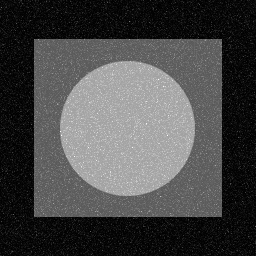
\includegraphics[width=\linewidth]{myfigure/p4/41-gaussian.png}
		\caption{}
		\label{fig:add_gaussian}
	\end{subfigure}
  	\begin{subfigure}[b]{0.25\linewidth}
		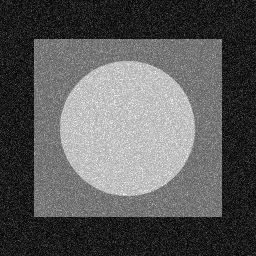
\includegraphics[width=\linewidth]{myfigure/p4/41-rayleigh.png}
		\caption{}
		\label{fig:add_rayleigh}
	\end{subfigure}
  	\begin{subfigure}[b]{0.25\linewidth}
		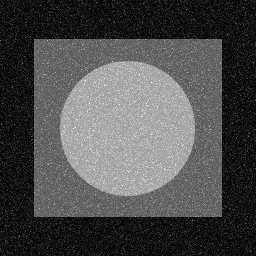
\includegraphics[width=\linewidth]{myfigure/p4/41-gamma.png}
		\caption{}
		\label{fig:add_gamma}
	\end{subfigure}
  	\begin{subfigure}[b]{0.25\linewidth}
		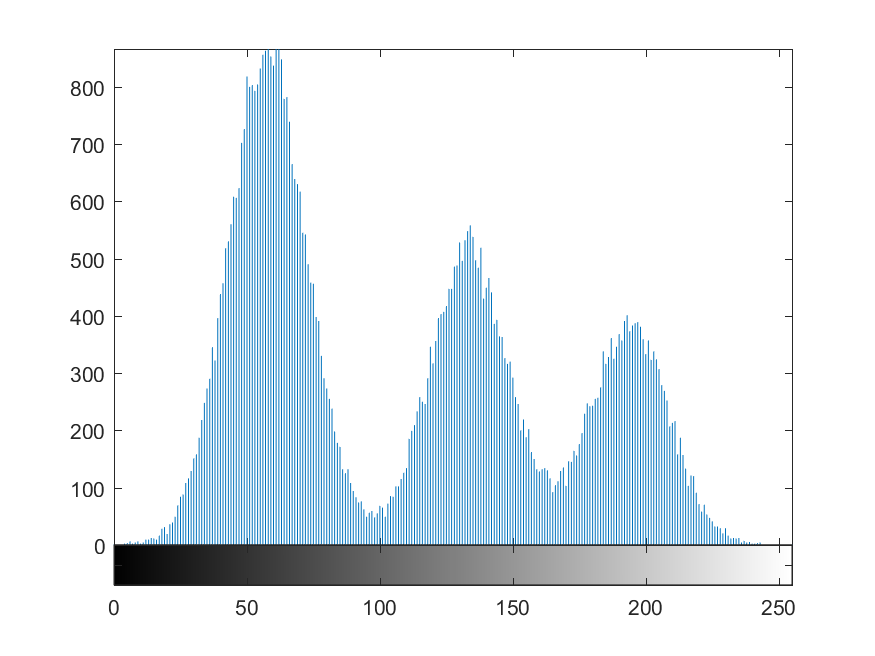
\includegraphics[width=\linewidth]{myfigure/p4/41-gaussian-hist.png}
		\caption{Gaussian}
		\label{fig:add_gaussian_hist}
	\end{subfigure}
  	\begin{subfigure}[b]{0.25\linewidth}
		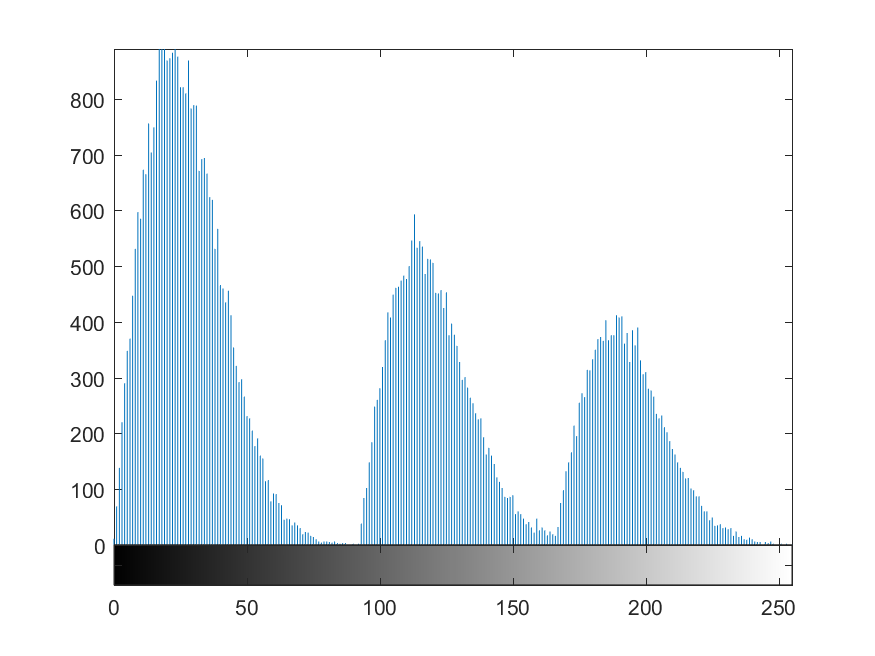
\includegraphics[width=\linewidth]{myfigure/p4/41-rayleigh-hist.png}
		\caption{Rayleigh}
		\label{fig:add_rayleigh_hist}
	\end{subfigure}
  	\begin{subfigure}[b]{0.25\linewidth}
		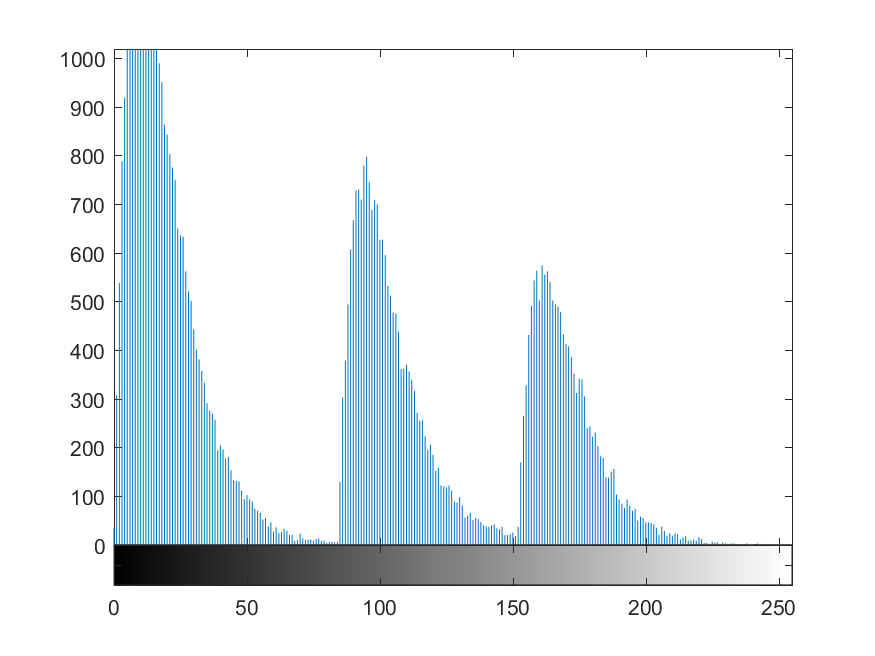
\includegraphics[width=\linewidth]{myfigure/p4/41-gamma-hist.png}
		\caption{Gamma}
		\label{fig:add_gamma_hist}
	\end{subfigure}
  	
  	\begin{subfigure}[b]{0.25\linewidth}
		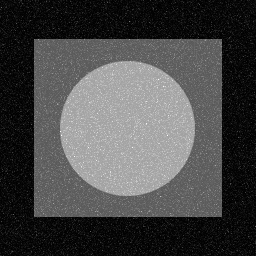
\includegraphics[width=\linewidth]{myfigure/p4/41-exp.png}
		\caption{}
		\label{fig:add_exp}
	\end{subfigure}
  	\begin{subfigure}[b]{0.25\linewidth}
		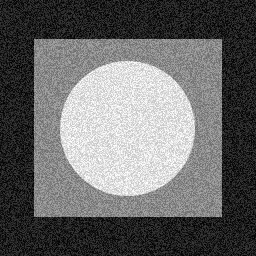
\includegraphics[width=\linewidth]{myfigure/p4/41-uniform.png}
		\caption{}
		\label{fig:add_uniform}
	\end{subfigure}
  	\begin{subfigure}[b]{0.25\linewidth}
		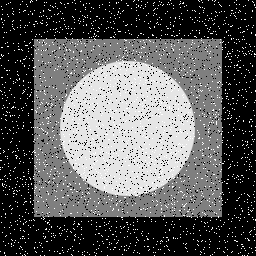
\includegraphics[width=\linewidth]{myfigure/p4/41-saltpepper.png}
		\caption{}
		\label{fig:add_saltpepper}
	\end{subfigure}
  	\begin{subfigure}[b]{0.25\linewidth}
		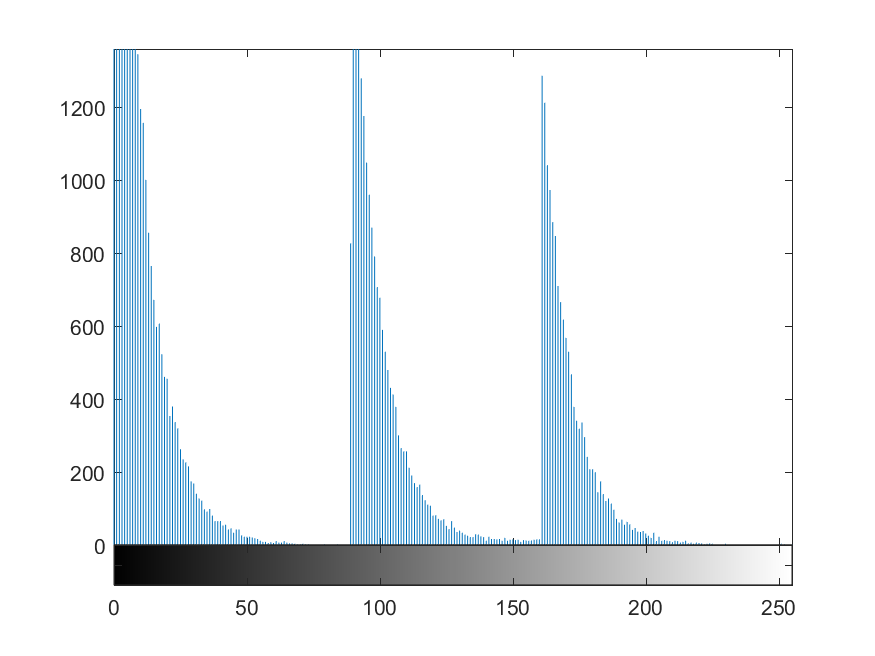
\includegraphics[width=\linewidth]{myfigure/p4/41-exp-hist.png}
		\caption{Exponential}
		\label{fig:add_exp_hist}
	\end{subfigure}
  	\begin{subfigure}[b]{0.25\linewidth}
		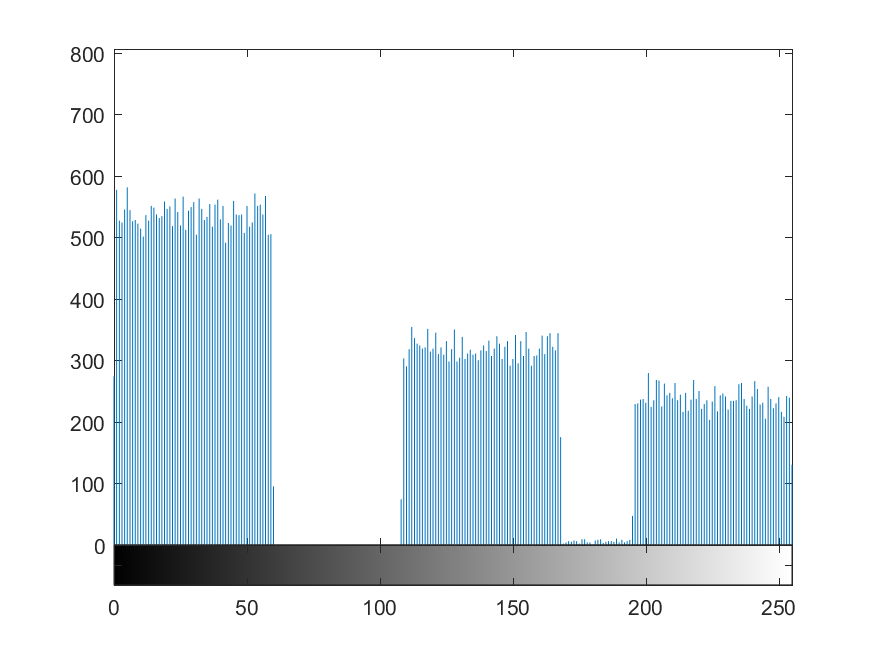
\includegraphics[width=\linewidth]{myfigure/p4/41-uniform-hist.png}
		\caption{Uniform}
		\label{fig:add_uniform_hist}
	\end{subfigure}
  	\begin{subfigure}[b]{0.25\linewidth}
		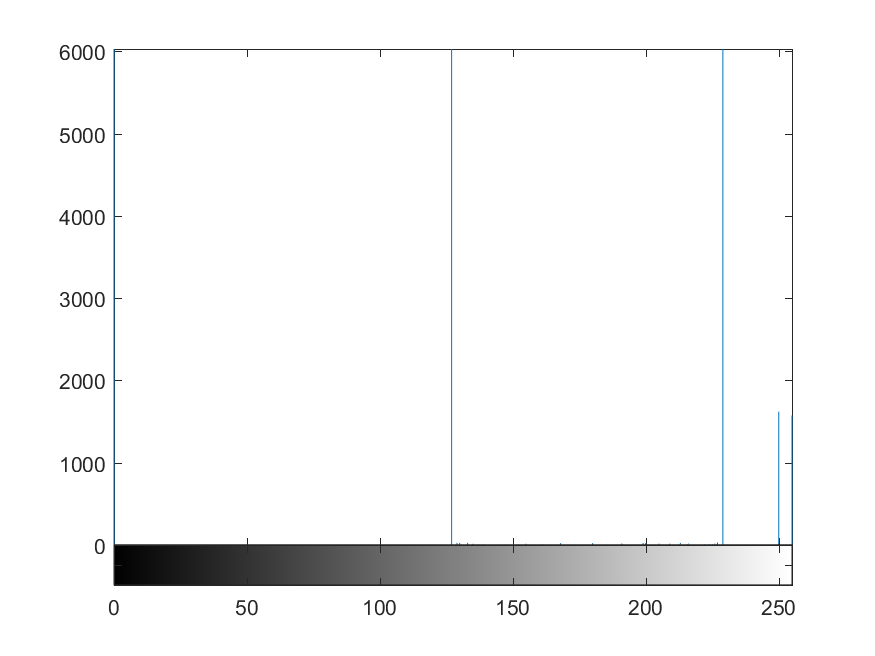
\includegraphics[width=\linewidth]{myfigure/p4/41-saltpepper-hist.png}
		\caption{Salt-and-pepper}
		\label{fig:add_saltpepper_hist}
	\end{subfigure}
  	\caption{(\ref{fig:orig})Original test image of size $688\times 688$ pixels. (\ref{fig:spectrum})Non-padded centered Fourier spectrum of the original test image.}
  	\label{fig:add_noise}
\end{figure}

\subsection{Experiment-2 Noise reduction}
\subsubsection{Follow fig5.7 in textbook}
The work in this part is shown in Figure.\ref{fig:5-7}. On the original X-ray image in Figure.\ref{fig:5-7a} of circuit board, we add Gaussian noise of $N(0,400)$. The corrupted image is shown in Figure.\ref{fig:5-7b}. In Figure.\ref{fig:5-7c}, we use $3\times3$ arithmetic mean filter to reduce the noise. In Figure.\ref{fig:5-7d} is the result of geometric mean filtering. We can see that both filters did a reasonable job of attenuating noise. Moreover, geometric mean filter performs better on Gaussian noise as it causes less blurring than arithmetic mean filter do.
\begin{figure}[h]
	\centering
	\begin{subfigure}[b]{0.4\linewidth}
		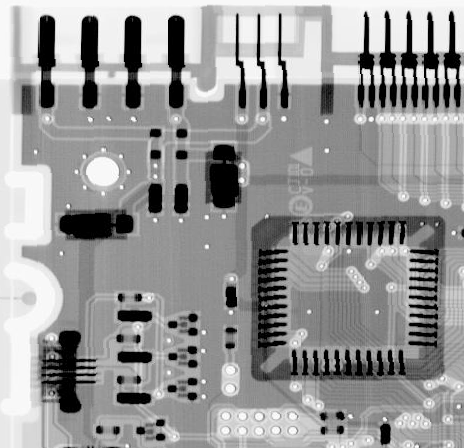
\includegraphics[width=\linewidth]{myfigure/p4/42-orig.png}
		\caption{}
		\label{fig:5-7a}
	\end{subfigure}
  	\begin{subfigure}[b]{0.4\linewidth}
		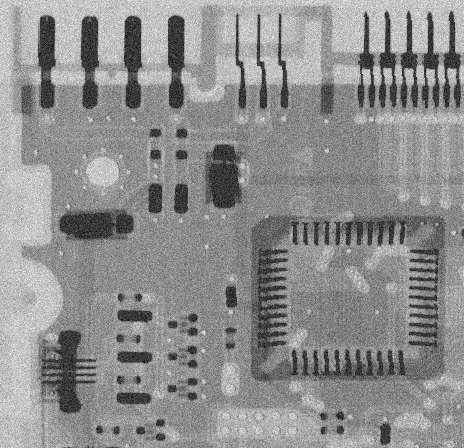
\includegraphics[width=\linewidth]{myfigure/p4/42-gaussian.png}
		\caption{}
		\label{fig:5-7b}
	\end{subfigure}
  	\begin{subfigure}[b]{0.4\linewidth}
		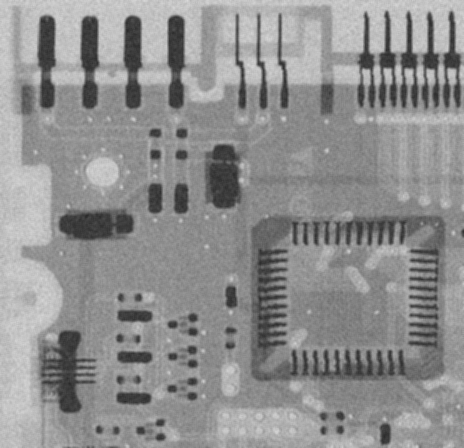
\includegraphics[width=\linewidth]{myfigure/p4/42-gau-arimean.png}
		\caption{}
		\label{fig:5-7c}
	\end{subfigure}
  	\begin{subfigure}[b]{0.4\linewidth}
		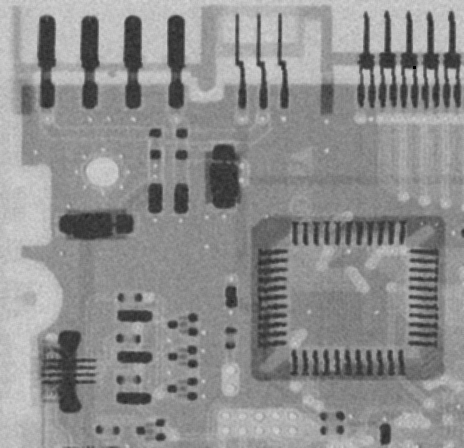
\includegraphics[width=\linewidth]{myfigure/p4/42-gau-geomean.png}
		\caption{}
		\label{fig:5-7d}
	\end{subfigure}
  	\caption{(\ref{fig:5-7a})Original image. (\ref{fig:5-7b})Add Gaussian noise $N(0,400)$. (\ref{fig:5-7c})Result of filtering with an arithmetic mean filter of size $3\times 3$. (\ref{fig:5-7d})Result of filtering with an geometric mean filter of size $3\times 3$}
  	\label{fig:5-7}
\end{figure}

\subsubsection{Follow fig5.8 in textbook}
The work in this part is shown in Figure.\ref{fig:5-8}. We add pepper noise and salt noise separately in Figure.\ref{fig:5-8a} and Figure.\ref{fig:5-8b} relatively. Then we use two $3\times 3$ contraharmonic mean filters with $Q=1.5$ and $Q=-1.5$ separately to pepper and salt noise relatively. The result is fine but we have to know the type of the noise, which is an ideal situation. 
\begin{figure}[h]
	\centering
	\begin{subfigure}[b]{0.4\linewidth}
		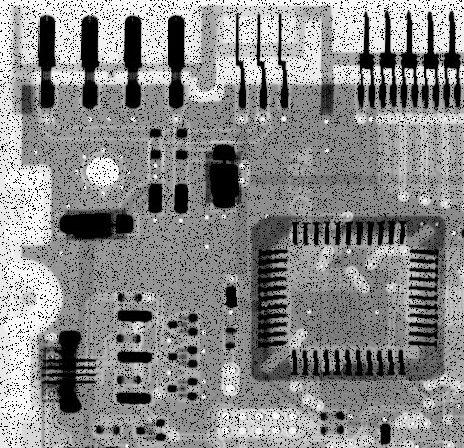
\includegraphics[width=\linewidth]{myfigure/p4/42-pepper.png}
		\caption{}
		\label{fig:5-8a}
	\end{subfigure}
	\begin{subfigure}[b]{0.4\linewidth}
		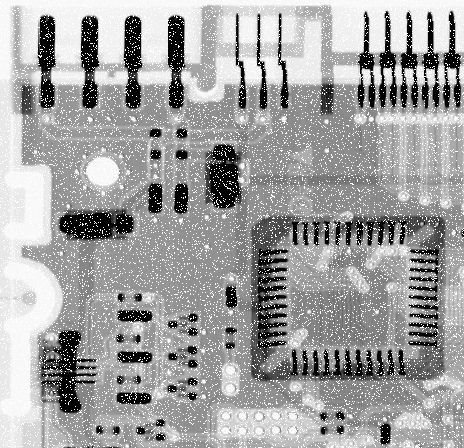
\includegraphics[width=\linewidth]{myfigure/p4/42-salt.png}
		\caption{}
		\label{fig:5-8b}
	\end{subfigure}
  	\begin{subfigure}[b]{0.4\linewidth}
		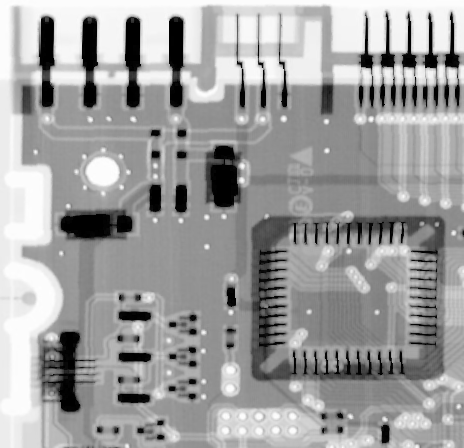
\includegraphics[width=\linewidth]{myfigure/p4/42-pepper-contraharmo.png}
		\caption{}
		\label{fig:5-8c}
	\end{subfigure}
  	\begin{subfigure}[b]{0.4\linewidth}
		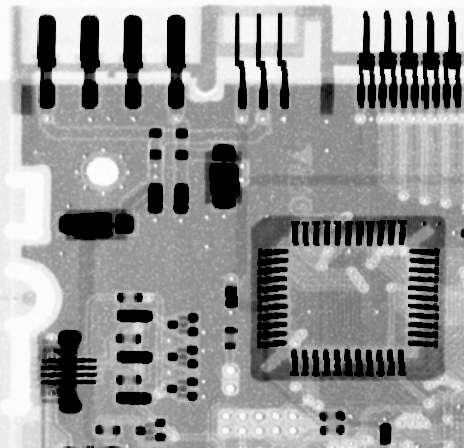
\includegraphics[width=\linewidth]{myfigure/p4/42-salt-contraharmo.png}
		\caption{}
		\label{fig:5-8d}
	\end{subfigure}
  	\caption{(\ref{fig:5-8a})Image corrupted by pepper noise with a probability of 0.1. (\ref{fig:5-8b})Image corrupted by salt noise with probability of 0.1. (\ref{fig:5-8c})Result of filtering \ref{fig:5-8a} with a $3\times 3$ contraharmonic filter of order $Q=1.5$ . (\ref{fig:5-8d})Result of filtering \ref{fig:5-8b} with $Q=-1.5$}
  	\label{fig:5-8}
\end{figure}

\subsubsection{Follow fig.5.9 in textbook}
The work in this part shows the wrong using of contraharmonic mean filter. If we use $Q=-1.5$ for pepper noise in Figure.\ref{fig:5-8a} and $Q=1.5$ for salt noise in Figure.\ref{fig:5-8b}, then we will get the bad results in Figure.\ref{fig:5-9a} and Figure.\ref{fig:5-9b} respectively.
\begin{figure}[h]
	\centering
	\begin{subfigure}[b]{0.4\linewidth}
		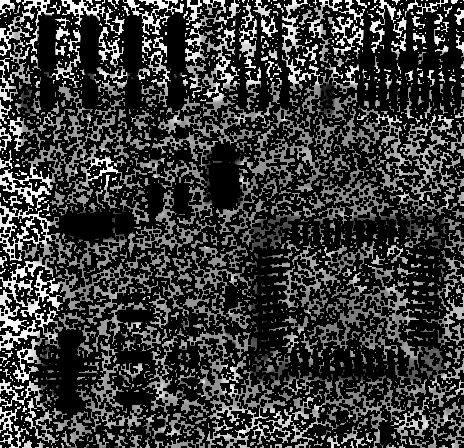
\includegraphics[width=\linewidth]{myfigure/p4/42-pepper-contraharmo_bad.png}
		\caption{}
		\label{fig:5-9a}
	\end{subfigure}
	\begin{subfigure}[b]{0.4\linewidth}
		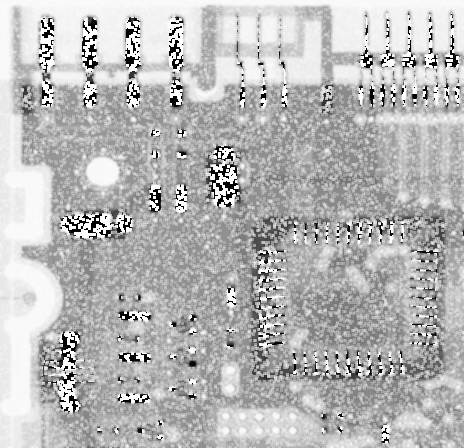
\includegraphics[width=\linewidth]{myfigure/p4/42-salt-contraharmo_bad.png}
		\caption{}
		\label{fig:5-9b}
	\end{subfigure}
  	\caption{(\ref{fig:5-9a})Use contraharmonic filter with $Q=-1.5$ for pepper noise in \ref{fig:5-8a}. (\ref{fig:5-9b}) Use contraharmonic filter with $Q=1.5$ for salt noise in \ref{fig:5-8b}.}
  	\label{fig:5-9}
\end{figure}

\subsubsection{Follow fig.5.10 in textbook}
Here we add salt noise and pepper noise with $P_a=P_b=0.1$ at the same time in Figure.\ref{fig:5-10a}. The we use $3\times 3$ median filter to filtering the image for 3 times and the result of each step is showed in Figure.\ref{fig:5-10b}, Figure.\ref{fig:5-10c} and Figure.\ref{fig:5-10d} respectively. We can see that the first time of filtering removes most of the noise and the next two times filtering get even better. The result is excellent as no blurring appears.
\begin{figure}[h]
	\centering
	\begin{subfigure}[b]{0.4\linewidth}
		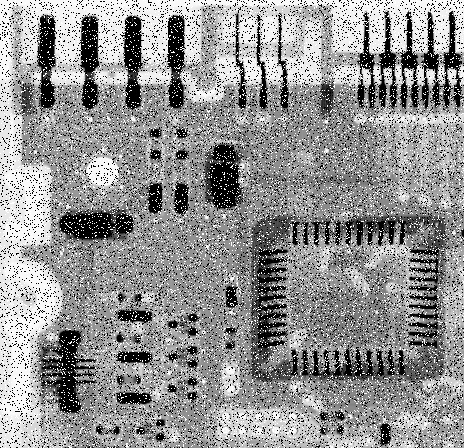
\includegraphics[width=\linewidth]{myfigure/p4/42-peppersalt.png}
		\caption{}
		\label{fig:5-10a}
	\end{subfigure}
	\begin{subfigure}[b]{0.4\linewidth}
		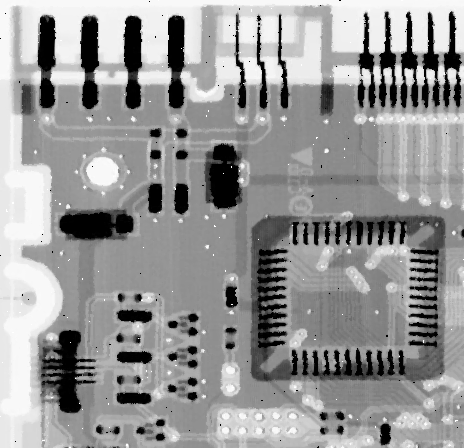
\includegraphics[width=\linewidth]{myfigure/p4/42-pepsalt-median-1.png}
		\caption{}
		\label{fig:5-10b}
	\end{subfigure}
  	\begin{subfigure}[b]{0.4\linewidth}
		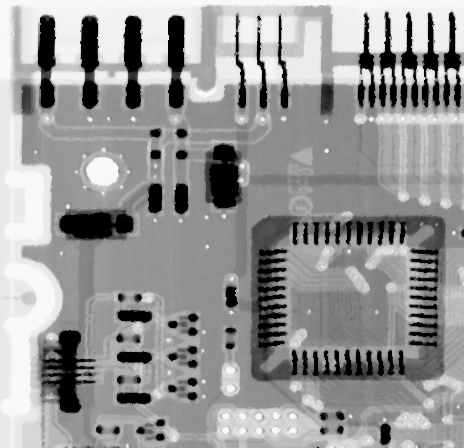
\includegraphics[width=\linewidth]{myfigure/p4/42-pepsalt-median-2.png}
		\caption{}
		\label{fig:5-10c}
	\end{subfigure}
  	\begin{subfigure}[b]{0.4\linewidth}
		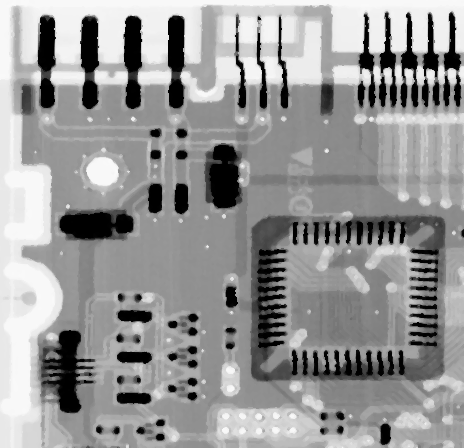
\includegraphics[width=\linewidth]{myfigure/p4/42-pepsalt-median-3.png}
		\caption{}
		\label{fig:5-10d}
	\end{subfigure}
  	\caption{(\ref{fig:5-10a})Add pepper noise and salt noise with $P_a=P_b=0.1$ at the same time to original image. (\ref{fig:5-10b})Apply $3\times 3$ median filter to \ref{fig:5-10a}.  (\ref{fig:5-10c})Apply the same filter to \ref{fig:5-10b}.  (\ref{fig:5-10d})Apply the same filter to \ref{fig:5-10c}. }
  	\label{fig:5-10}
\end{figure}

\subsubsection{Follow fig.5.11 in textbook}
In last part, we have see the power of order-statistic filter in pepper-and-salt noise reduction. Here, we use max filter for Figure.\ref{fig:5-8a} and min filter for Figure.\ref{fig:5-8b}. The result is also excellent because there is no import of blurring as well as thorough reduction of noise.
\begin{figure}[h]
	\centering
	\begin{subfigure}[b]{0.4\linewidth}
		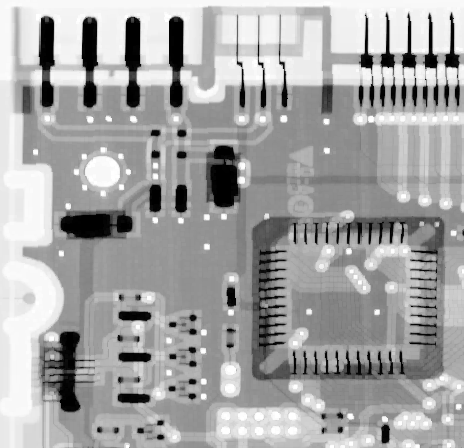
\includegraphics[width=\linewidth]{myfigure/p4/42-pepper-max.png}
		\caption{}
		\label{fig:5-11a}
	\end{subfigure}
	\begin{subfigure}[b]{0.4\linewidth}
		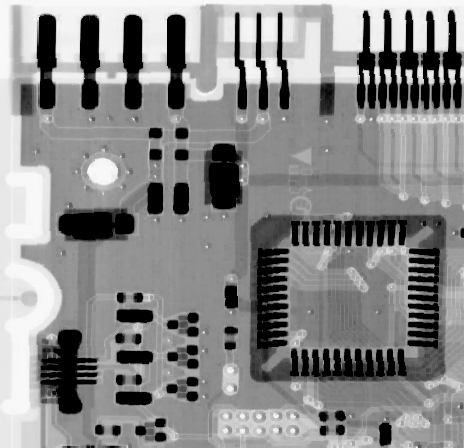
\includegraphics[width=\linewidth]{myfigure/p4/42-salt-min.png}
		\caption{}
		\label{fig:5-11b}
	\end{subfigure}
  	\caption{(\ref{fig:5-11a})Use max filter on \ref{fig:5-8a} (\ref{fig:5-11b}) Use min filter on \ref{fig:5-8b}.}
  	\label{fig:5-11}
\end{figure}

\subsubsection{Follow fig.5.12 in textbook}
In this part, we add uniform of zero mean and variance 800 and peper-and-salt with noise $P_a=P_b=0.1$ at the same time in Figure.\ref{fig:5-12b}. Then we apply 4 kinds of filter of size $5\times5$ to reduce noise. In Figure.\ref{fig:5-12c},\ref{fig:5-12d},\ref{fig:5-12e},\ref{fig:5-12f}, arithmetic mean filter, geometric mean filter, median filter, and alpha-trimmed filter with $d=5$ are used respectively. The two mean filter do not perform well as there are pepper-and-salt noise and the two order statistic filter do much better. However there are still some blurring due to the presence of uniform noise. The alpha-trimmed filter gets smoother results than median filter because it can remove the polar value which may contains much pepper-and-salt noise.
\begin{figure}[h]
	\centering
	\begin{subfigure}[b]{0.4\linewidth}
		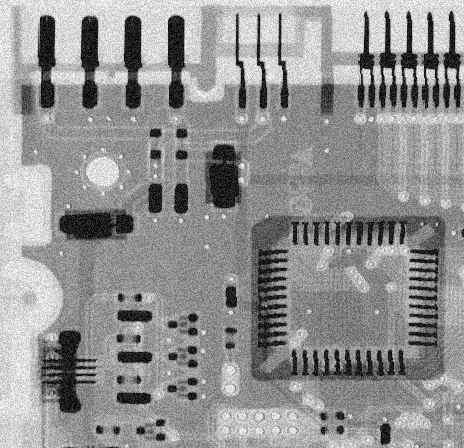
\includegraphics[width=\linewidth]{myfigure/p4/42-uniform.png}
		\caption{}
		\label{fig:5-12a}
	\end{subfigure}
	\begin{subfigure}[b]{0.4\linewidth}
		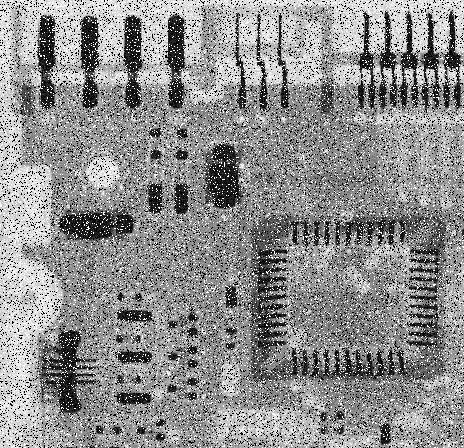
\includegraphics[width=\linewidth]{myfigure/p4/42-unipepsalt.png}
		\caption{}
		\label{fig:5-12b}
	\end{subfigure}
  	\begin{subfigure}[b]{0.4\linewidth}
		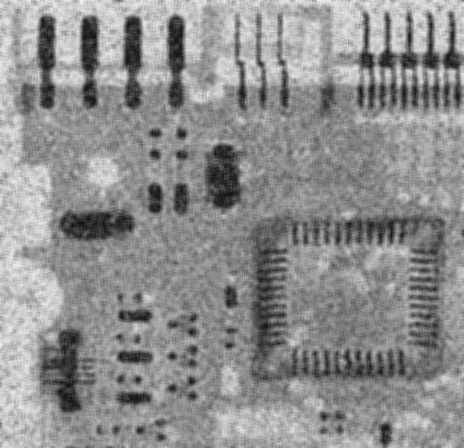
\includegraphics[width=\linewidth]{myfigure/p4/42-unipepsalt-arimean.png}
		\caption{}
		\label{fig:5-12c}
	\end{subfigure}
  	\begin{subfigure}[b]{0.4\linewidth}
		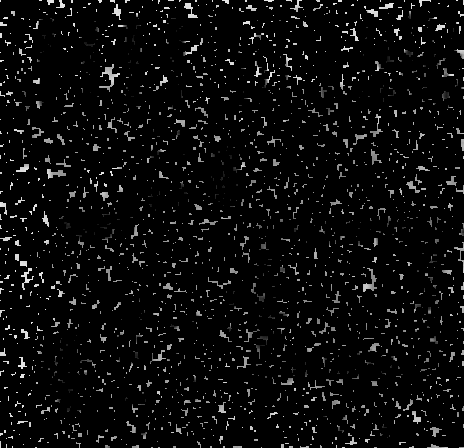
\includegraphics[width=\linewidth]{myfigure/p4/42-unipepsalt-geomean.png}
		\caption{}
		\label{fig:5-12d}
	\end{subfigure}
	\begin{subfigure}[b]{0.4\linewidth}
		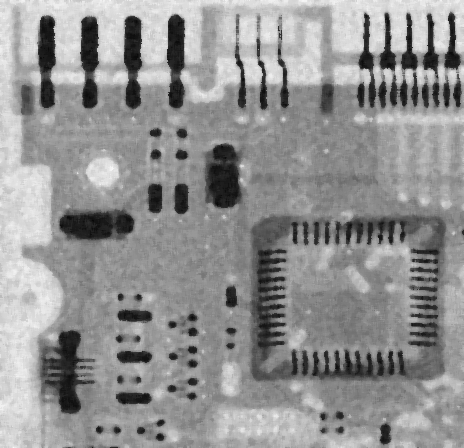
\includegraphics[width=\linewidth]{myfigure/p4/42-unipepsalt-median.png}
		\caption{}
		\label{fig:5-12e}
	\end{subfigure}
	\begin{subfigure}[b]{0.4\linewidth}
		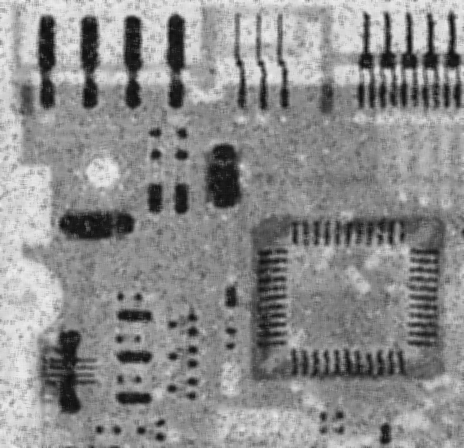
\includegraphics[width=\linewidth]{myfigure/p4/42-unipepsalt-alpha.png}
		\caption{}
		\label{fig:5-12f}
	\end{subfigure}
  	\caption{(\ref{fig:5-12a})Image corrupted by uniform noise of $U(0,800)$. (\ref{fig:5-12b})Image corrupted by pepper-and-salt noise with $P_a=P_b=0.1$. (\ref{fig:5-12c})Result of $5\times5$ arithmetic mean filtering. (\ref{fig:5-12d}) Result of $5\times5$ geometric mean filtering  (\ref{fig:5-12e})Result of $5\times5$ median filtering. (\ref{fig:5-12f})Result of $5\times5$ alpha-trimmed filtering with $d=5$.}
  	\label{fig:5-12}
\end{figure}

\clearpage
\subsection{Implementation}
The key points of implementation here are (1)the generation of different distribution from uniform distribution and (2)the implementation of different filters. All of these are listed in the following code piece.

\lstset{language=Matlab}
\begin{lstlisting}
function [ n_gaussian ] = gen_gaussian( mu, variance, M, N )
%GEN_GAUSSIAN 
%   generate gaussian distribution from uniform distribution
n_gaussian = zeros(M, N);
for i = (1:M)
    for j = (1:N)
        x1 = rand();
        x2 = rand();
        n_gaussian(i,j) = sqrt(-2 * log(x1))*cos(2*pi*x2);
    end
end
n_gaussian = n_gaussian * variance + mu;
end
\end{lstlisting}

\begin{lstlisting}
function [ n_rayleigh ] = gen_rayleigh( lowbound, variance, M, N )
%GEN_RAYLEIGH 
%   generate rayleigh distribution from uniform distribution
n_rayleigh = zeros(M, N);
for i = (1:M)
    for j = (1:N)
        x = rand();
        n_rayleigh(i, j) = sqrt(-2 * variance^2 * log(1-x));
    end
end
n_rayleigh = n_rayleigh + lowbound;
end
\end{lstlisting}

\begin{lstlisting}
function [ n_gamma ] = gen_gamma( gamma_a, gamma_b, M, N )
%GEN_GAMMA
%   generate gamma distribution from uniform distribution
n_gamma = zeros(M, N);
for i = (1:M)
    for j = (1:N)
        x = rand(1, gamma_b);
        x = log(1-x);
        n_gamma(i,j) = -1/gamma_a * sum(x);
    end
end
end
\end{lstlisting}

\begin{lstlisting}
function [ n_exp ] = gen_exp( exp_lambda, M, N )
%GEN_EXP 
%   generate exponential distribution from uniform distribution
n_exp = zeros(M, N);
for i = (1:M)
    for j = (1:N)
        x = rand();
        n_exp(i, j) = -1.0 / exp_lambda * log(1-x);
    end
end
end
\end{lstlisting}

\begin{lstlisting}
function [ n_saltpepper ] = gen_saltpepper( salt, pepper, p_salt, p_pepper, M, N )
%GEN_SALTPEPPER 
%   
n_saltpepper  = zeros(M, N);
for i = (1:M)
    for j = (1:N)
        x = rand();
        if x < p_salt
            n_saltpepper(i, j) = salt;
        else
            if x < p_salt + p_pepper
                n_saltpepper(i, j) = pepper;
            end
        end
    end
end

end

\end{lstlisting}

\begin{lstlisting}
function [ imgg ] = arithmetic_mean( imgf, p )
%ARITHMIC_MEAN 
%   
[M, N] = size(imgf);
f = replicate_padding(imgf, p-1);
f = double(f);
g = zeros(M+p-1, N+p-1);
for i = ((p+1)/2:M+p-1+(p-1)/2)
    for j = ((p+1)/2:N+p-1+(p-1)/2)
        g(i, j) = sum(sum(f(i-(p-1)/2:i+(p-1)/2, j-(p-1)/2:j+(p-1)/2))) / p / p;
    end
end
imgg = uint8(g(p:M+p-1, p:N+p-1));
end
\end{lstlisting}

\begin{lstlisting}
function [ imgg ] = geometric_mean( imgf, p )
%GEOMETRY_MEAN
%   
[M, N] = size(imgf);
f = replicate_padding(imgf, p-1);
f = double(f);
g = zeros(M+p-1, N+p-1);
for i = ((p+1)/2:M+p-1+(p-1)/2)
    for j = ((p+1)/2:N+p-1+(p-1)/2)
        g(i, j) = (prod(prod(f(i-(p-1)/2:i+(p-1)/2, j-(p-1)/2:j+(p-1)/2)))) ^ (1/p/p) ;
    end
end
imgg = uint8(g(p:M+p-1, p:N+p-1));
end
\end{lstlisting}

\begin{lstlisting}
function [ imgg ] = contra_harmonic( imgf, p, Q )
%CONTRA_HARMONIC 
%   
[M, N] = size(imgf);
f = replicate_padding(imgf, p-1);
f = double(f);
g = zeros(M+p-1, N+p-1);
for i = ((p+1)/2:M+p-1+(p-1)/2)
    for j = ((p+1)/2:N+p-1+(p-1)/2)
        g(i, j) = sum(sum(f(i-(p-1)/2:i+(p-1)/2, j-(p-1)/2:j+(p-1)/2) .^ (Q+1))) / ...
                    sum(sum(f(i-(p-1)/2:i+(p-1)/2, j-(p-1)/2:j+(p-1)/2) .^ Q));
    end
end
imgg = scale255(g(p:M+p-1, p:N+p-1));
imgg = uint8(imgg);
end
\end{lstlisting}

\begin{lstlisting}
function [ imgg ] = median_spatial( imgf, p )
%MEDIAN 
%   
[M, N] = size(imgf);
f = replicate_padding(imgf, p-1);
f = double(f);
g = zeros(M+p-1, N+p-1);
for i = ((p+1)/2:M+p-1+(p-1)/2)
    for j = ((p+1)/2:N+p-1+(p-1)/2)
        spatial = f(i-(p-1)/2:i+(p-1)/2, j-(p-1)/2:j+(p-1)/2);
        g(i, j) = median(spatial(:));
    end
end
imgg = uint8(g(p:M+p-1, p:N+p-1));

end
\end{lstlisting}

\begin{lstlisting}
function [ imgg ] = max_spatial( imgf, p )
%MAX_SPATIAL
%
[M, N] = size(imgf);
f = replicate_padding(imgf, p-1);
f = double(f);
g = zeros(M+p-1, N+p-1);
for i = ((p+1)/2:M+p-1+(p-1)/2)
    for j = ((p+1)/2:N+p-1+(p-1)/2)
        spatial = f(i-(p-1)/2:i+(p-1)/2, j-(p-1)/2:j+(p-1)/2);
        g(i, j) = max(spatial(:));
    end
end
imgg = uint8(g(p:M+p-1, p:N+p-1));
end
\end{lstlisting}

\begin{lstlisting}
function [ imgg ] = alpha_trimmed( imgf, p, d )
%ALPHA_TRIMMED 
%   
[M, N] = size(imgf);
f = replicate_padding(imgf, p-1);
f = double(f);
g = zeros(M+p-1, N+p-1);
for i = ((p+1)/2:M+p-1+(p-1)/2)
    for j = ((p+1)/2:N+p-1+(p-1)/2)
        t = f(i-(p-1)/2:i+(p-1)/2, j-(p-1)/2:j+(p-1)/2);
        tt = sort(t(:));
        g(i, j) = sum(tt( fix(d/2)+1 : p*p-(d-fix(d/2)) )) / (p*p - d);
    end
end
imgg = uint8(g(p:M+p-1, p:N+p-1));

end
\end{lstlisting}

